A quick way to access the Table~\ref{function_values:pressure_vessel_problem} is shown on Figure~\ref{fig:pressure_vessel_design_boxplot}.

\begin{figure}[H]
\centering
\caption{Boxplot for Pressure Vessel Design}
\label{fig:pressure_vessel_design_boxplot}
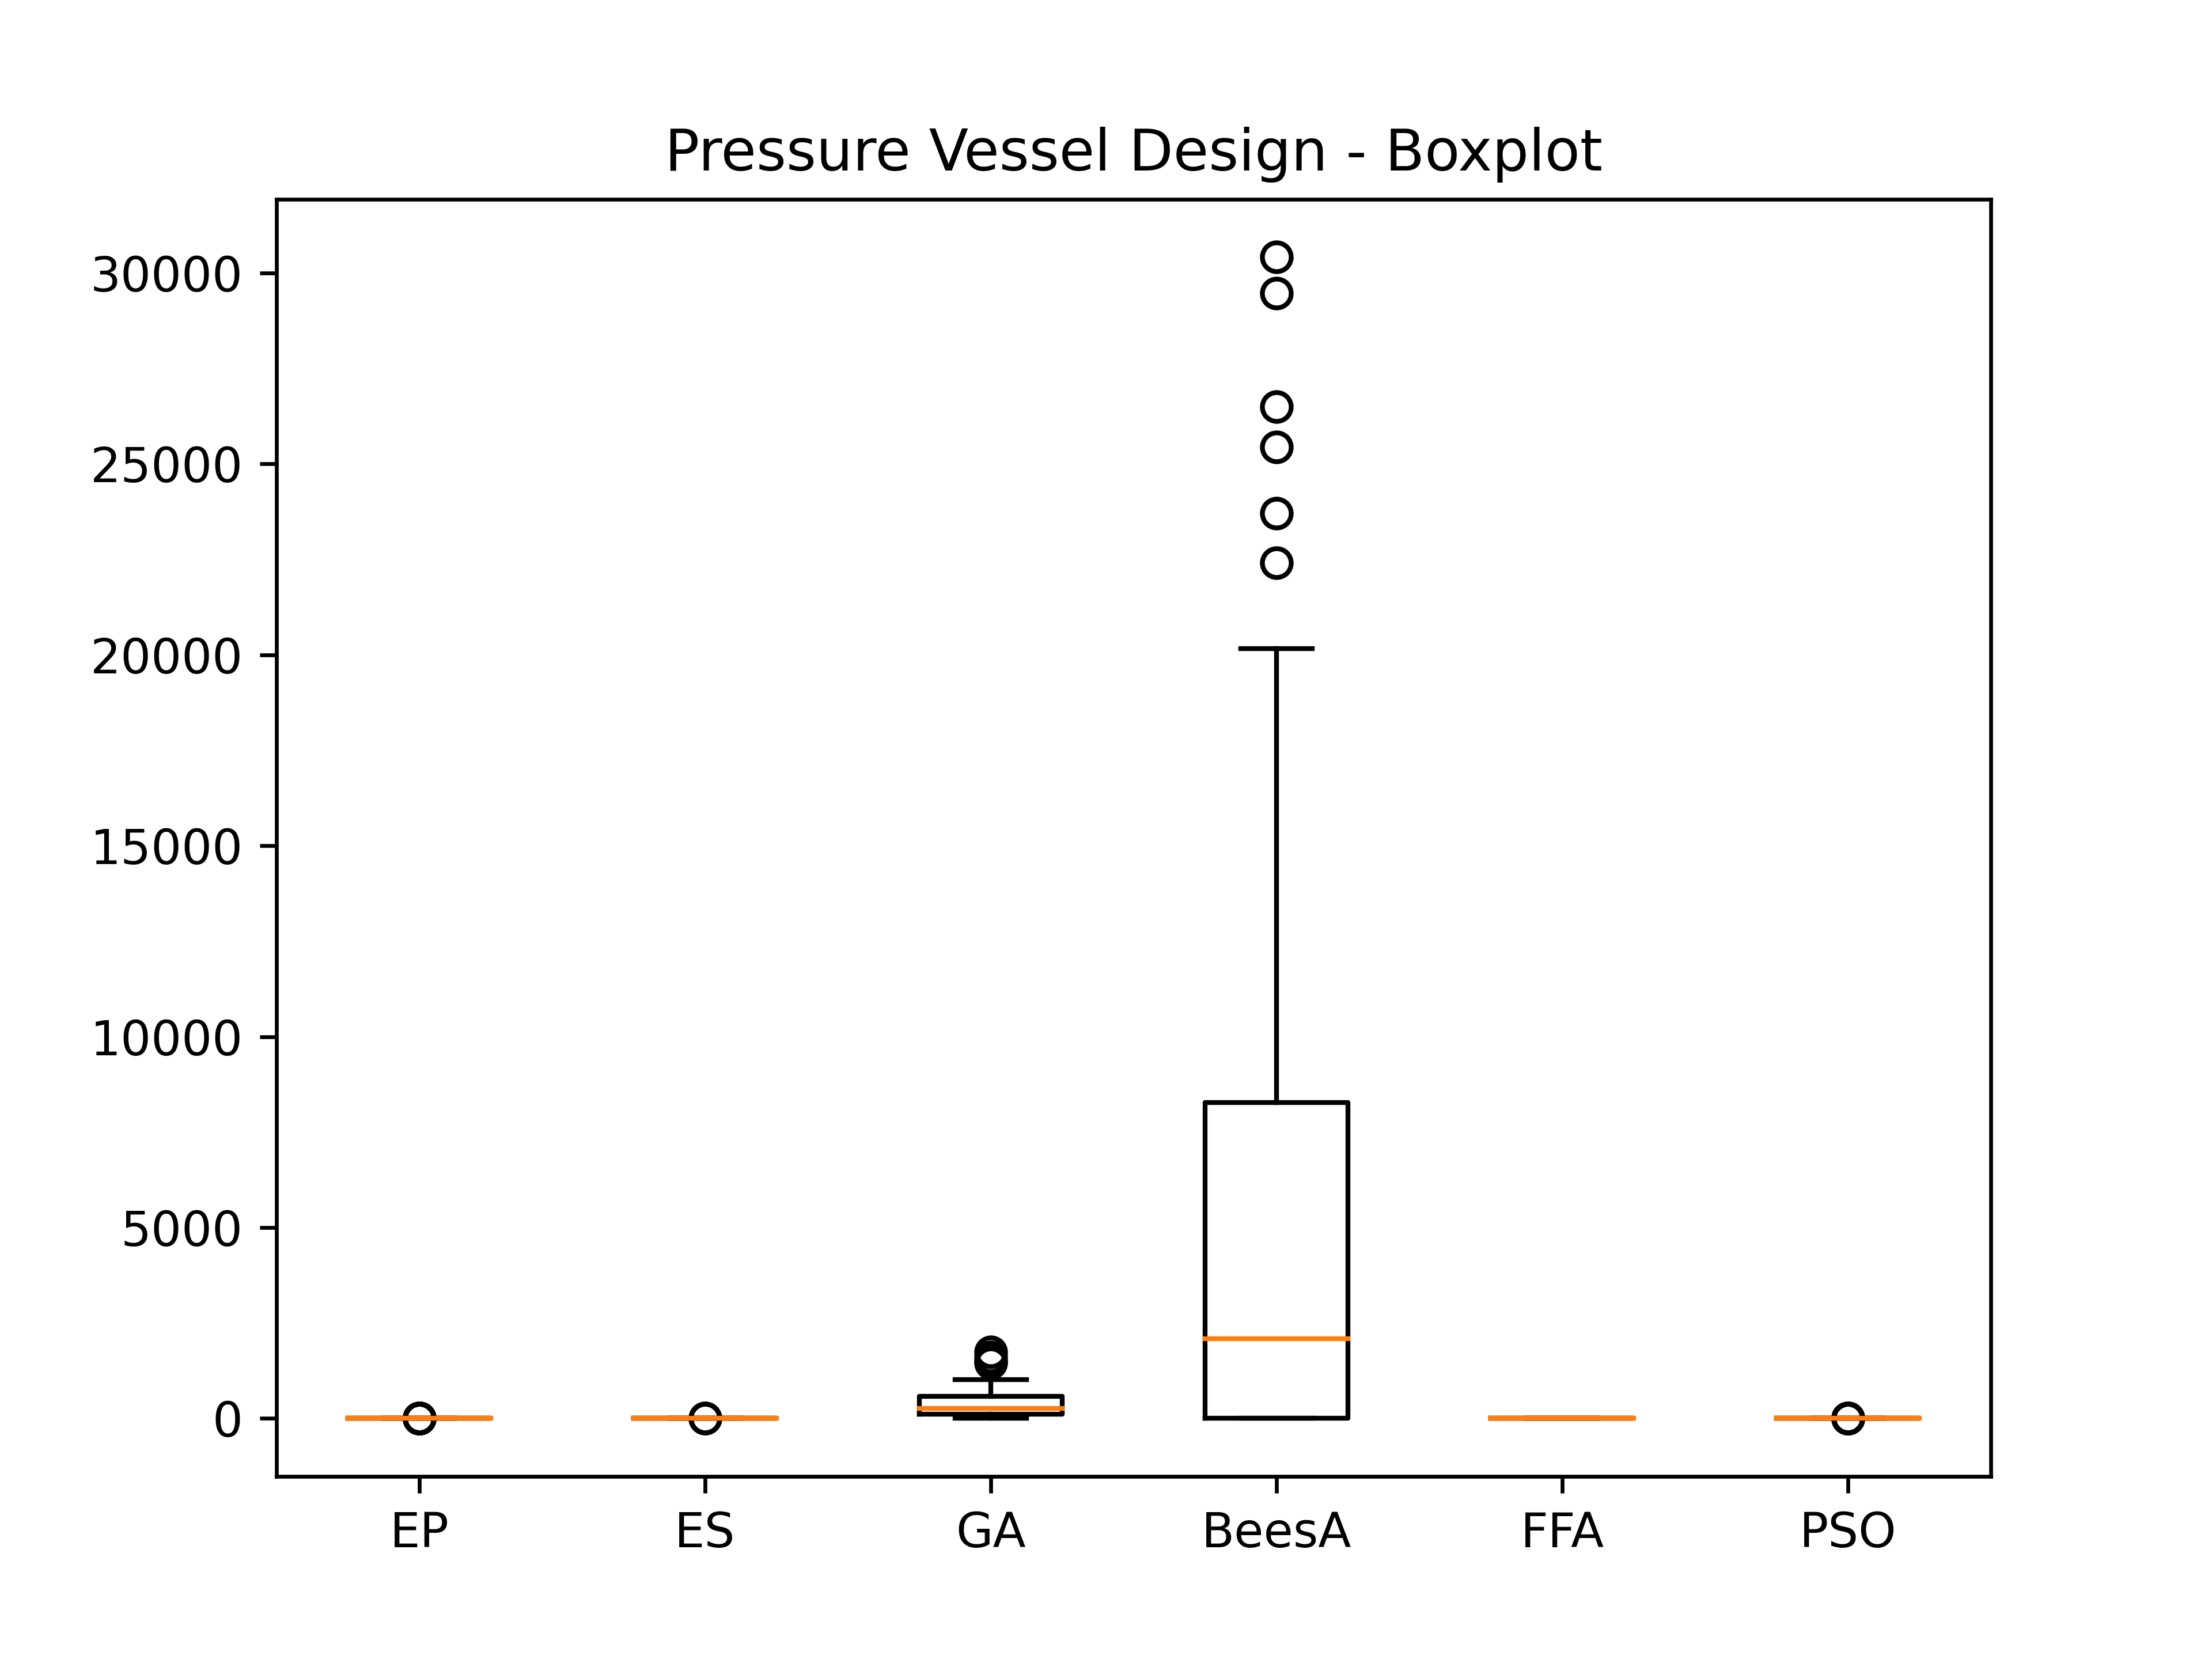
\includegraphics[scale=0.5]{images/pressure_vessel_problem_boxplot.png}
\end{figure}

It shows the same information as the Table~\ref{function_values:pressure_vessel_problem}
and it evidences that not all algorithms have the same mean, so it is a clear evidence
that not all algorithm give similar results from an arbitrary start point.